\documentclass{article}[11pt]

\usepackage{amsmath}
\usepackage{amsfonts}

\usepackage{graphicx}
\graphicspath{{../data/}} 								% Path to a folder where all pictures are located

\usepackage{fullpage}

\title{Machine Learning -- Assignment 6}
\author{Weipeng He \texttt{6411529} \\ \texttt{2he@informatik.uni-hamburg.de}  \\ with Jyothi Yalpi and Sathya Narayanan}

\begin{document}

\maketitle

\section{}
\paragraph{Data without noise}
\begin{enumerate}
\item 
Linear kernel with $C=100$
\begin{center}
  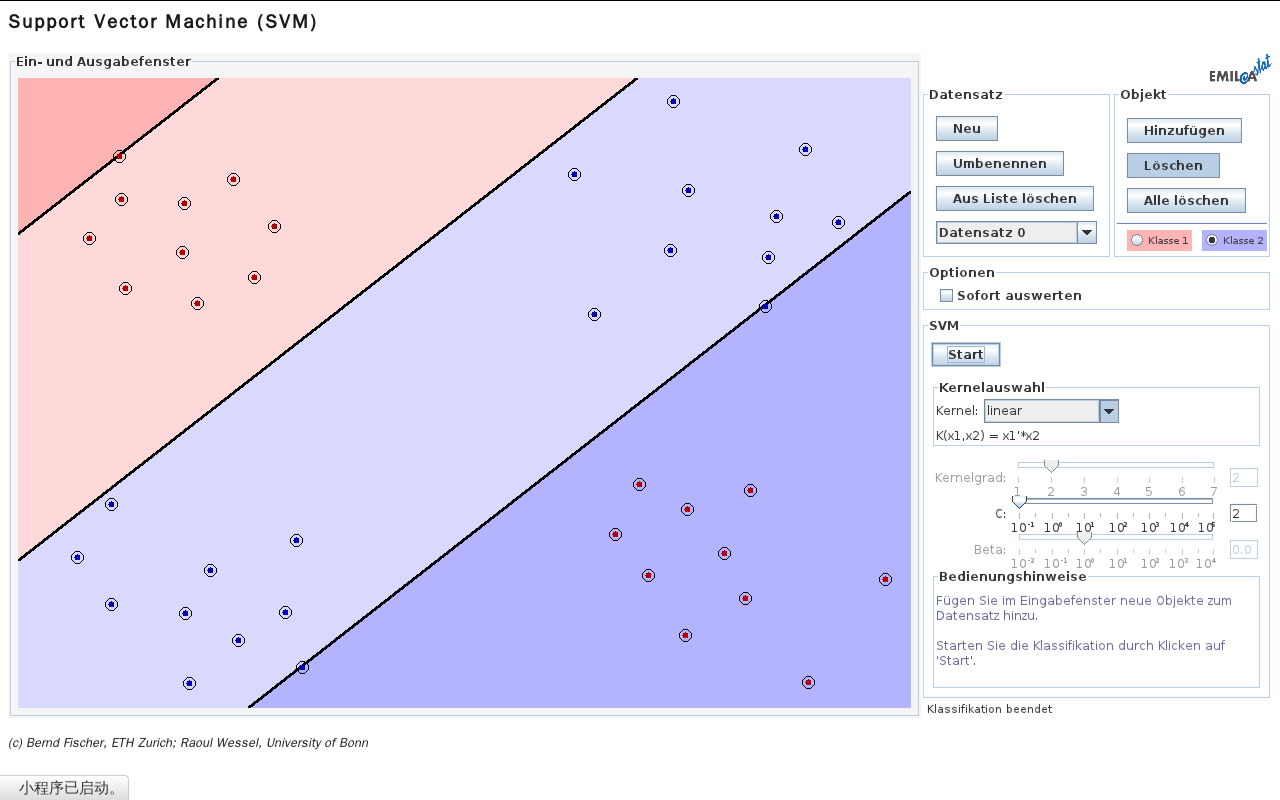
\includegraphics[width=.9\textwidth]{a-lin-c2}
\end{center}

\item 
Polynomial kernel with degree $2$ and $C=10$
\begin{center}
  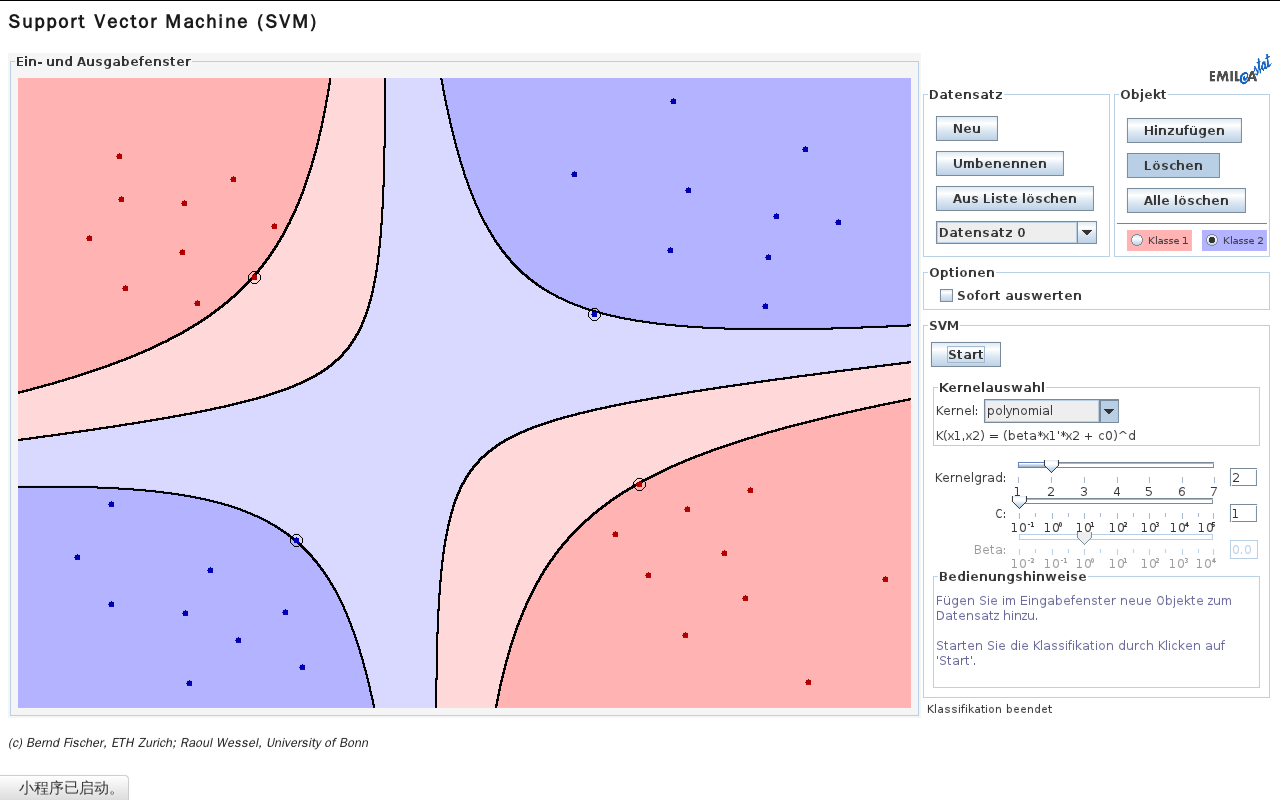
\includegraphics[width=.9\textwidth]{a-poly2-c1}
\end{center}

\item 
Polynomial kernel with degree $8$ and $C=10$
\begin{center}
  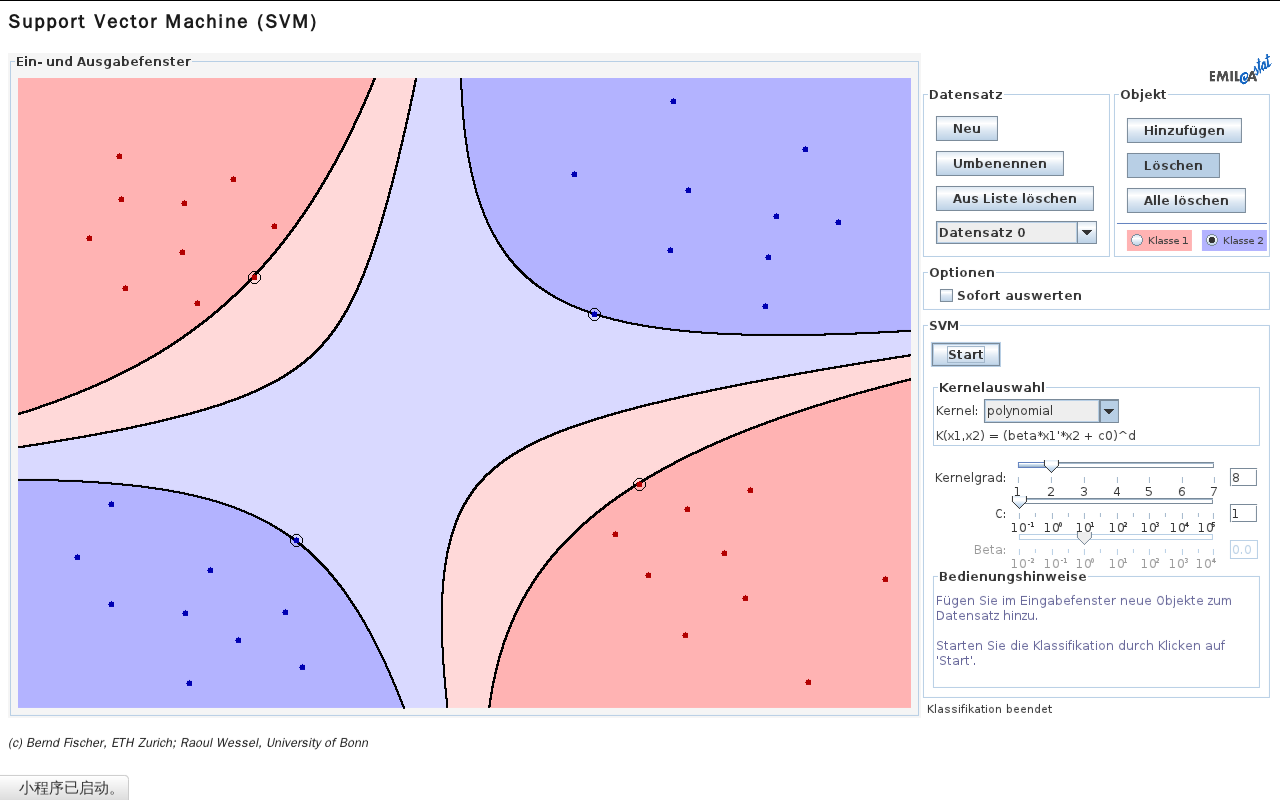
\includegraphics[width=.9\textwidth]{a-poly8-c1}
\end{center}

\item 
Gaussian kernel with $\beta = 0.01$ and $C=10^5$
\begin{center}
  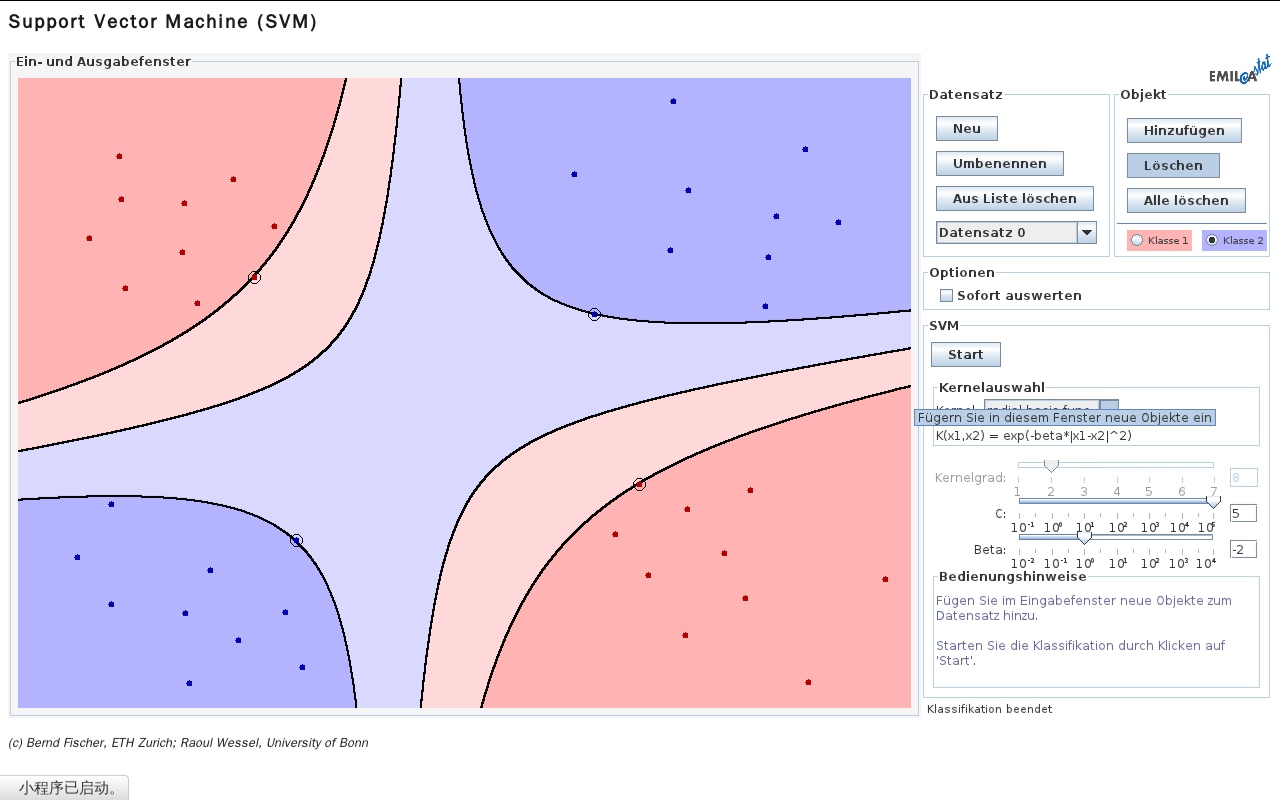
\includegraphics[width=.9\textwidth]{a-rbf-b-2-c5}
\end{center}

\item 
Gaussian kernel with $\beta = 1$ and $C=10$
\begin{center}
  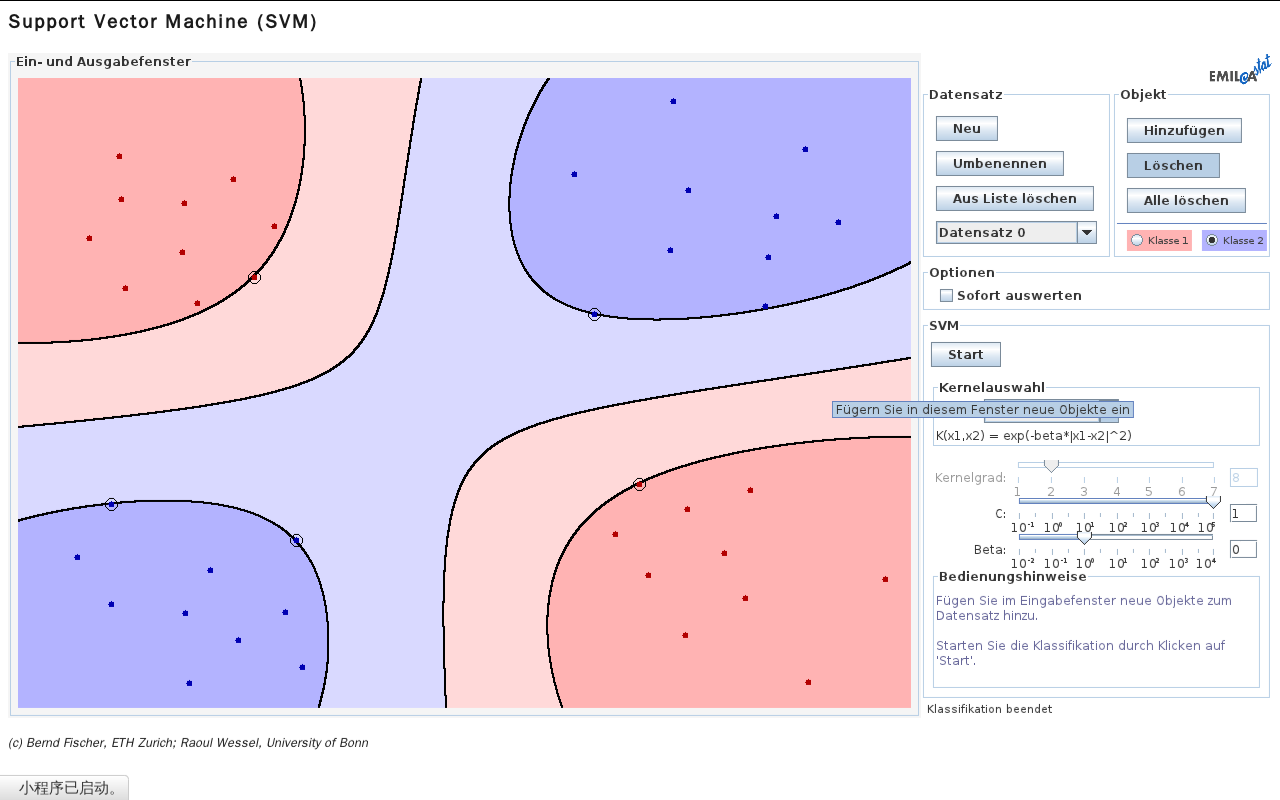
\includegraphics[width=.9\textwidth]{a-rbf-b0-c1}
\end{center}

\item 
Gaussian kernel with $\beta = 10$ and $C=10$
\begin{center}
  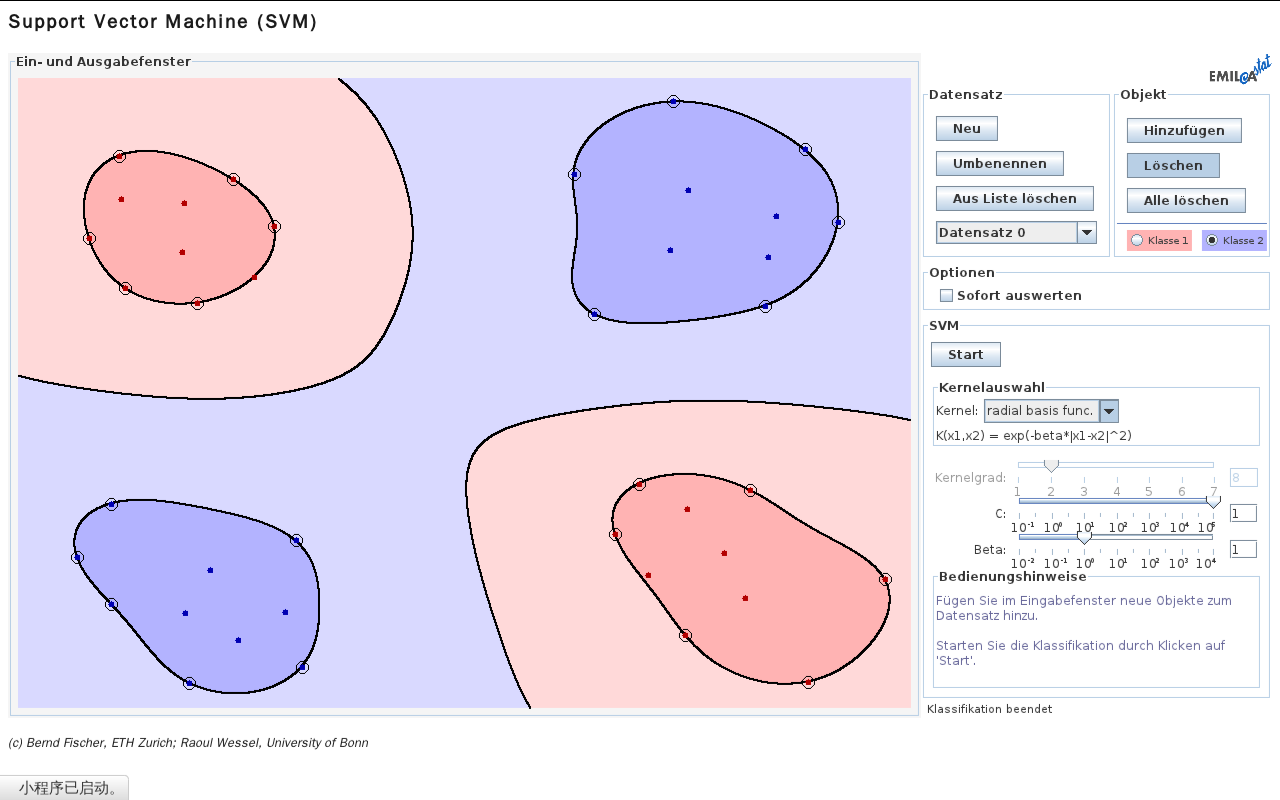
\includegraphics[width=.9\textwidth]{a-rbf-b1-c1}
\end{center}

\item 
Gaussian kernel with $\beta = 100$ and $C=10$
\begin{center}
  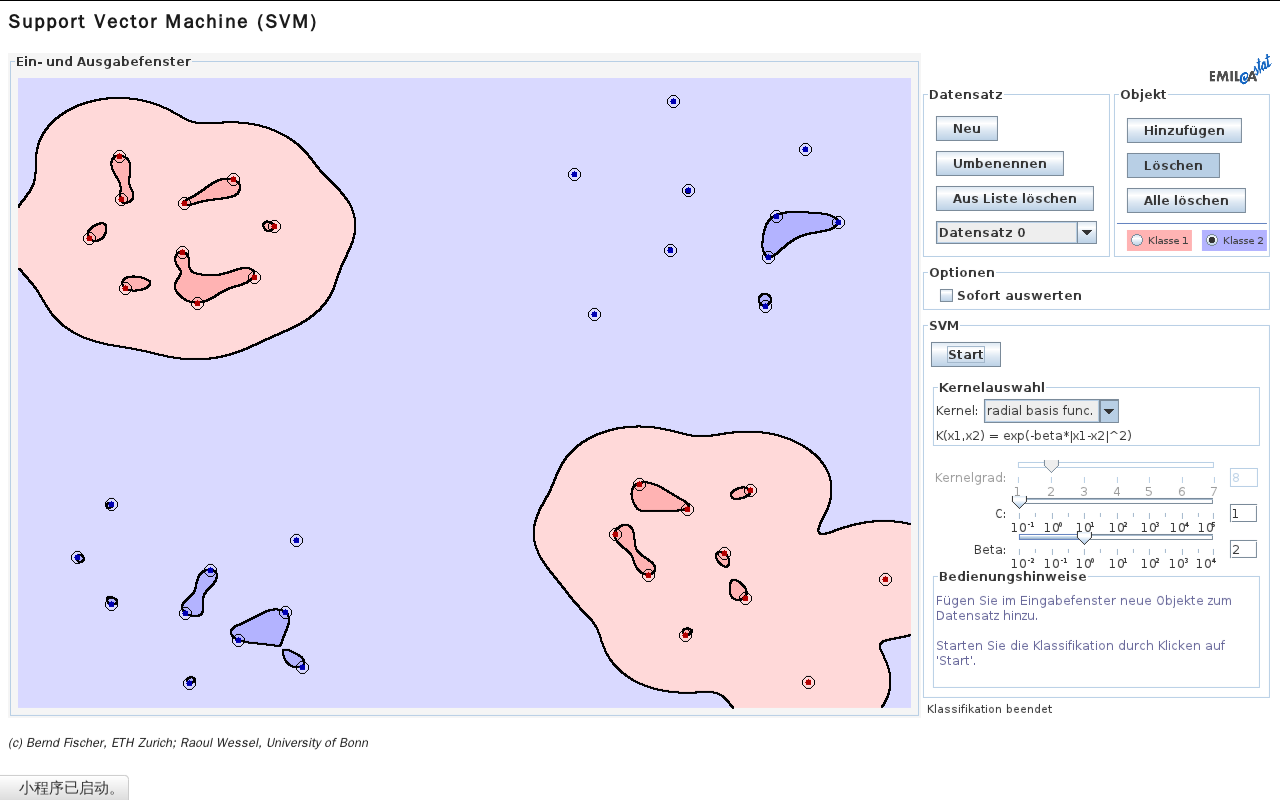
\includegraphics[width=.9\textwidth]{a-rbf-b2-c1}
\end{center}

\end{enumerate}
\paragraph{Data with noise}
\begin{enumerate}
\item 
Gaussian kernel with $\beta = 10$ and $C=0.01$
\begin{center}
  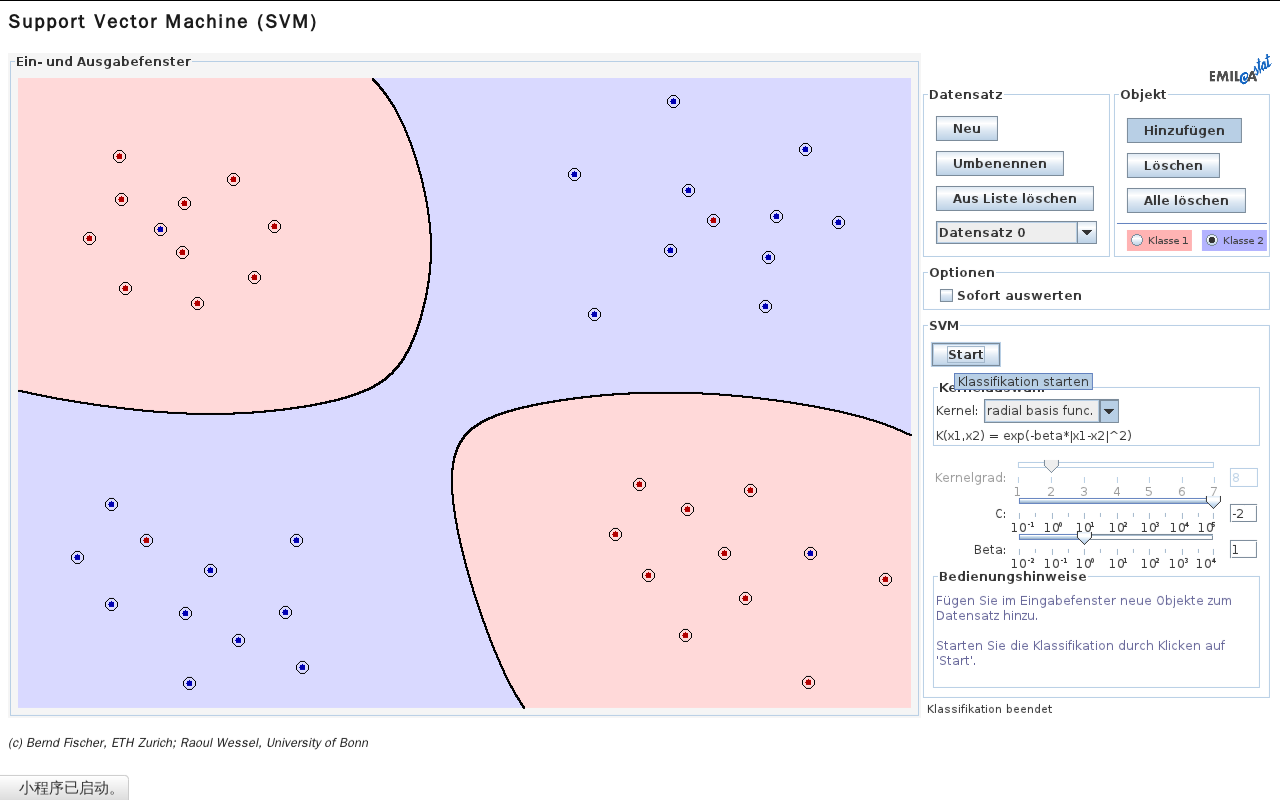
\includegraphics[width=.9\textwidth]{b-rbf-b1-c-2}
\end{center}

\item 
Gaussian kernel with $\beta = 10$ and $C=10$
\begin{center}
  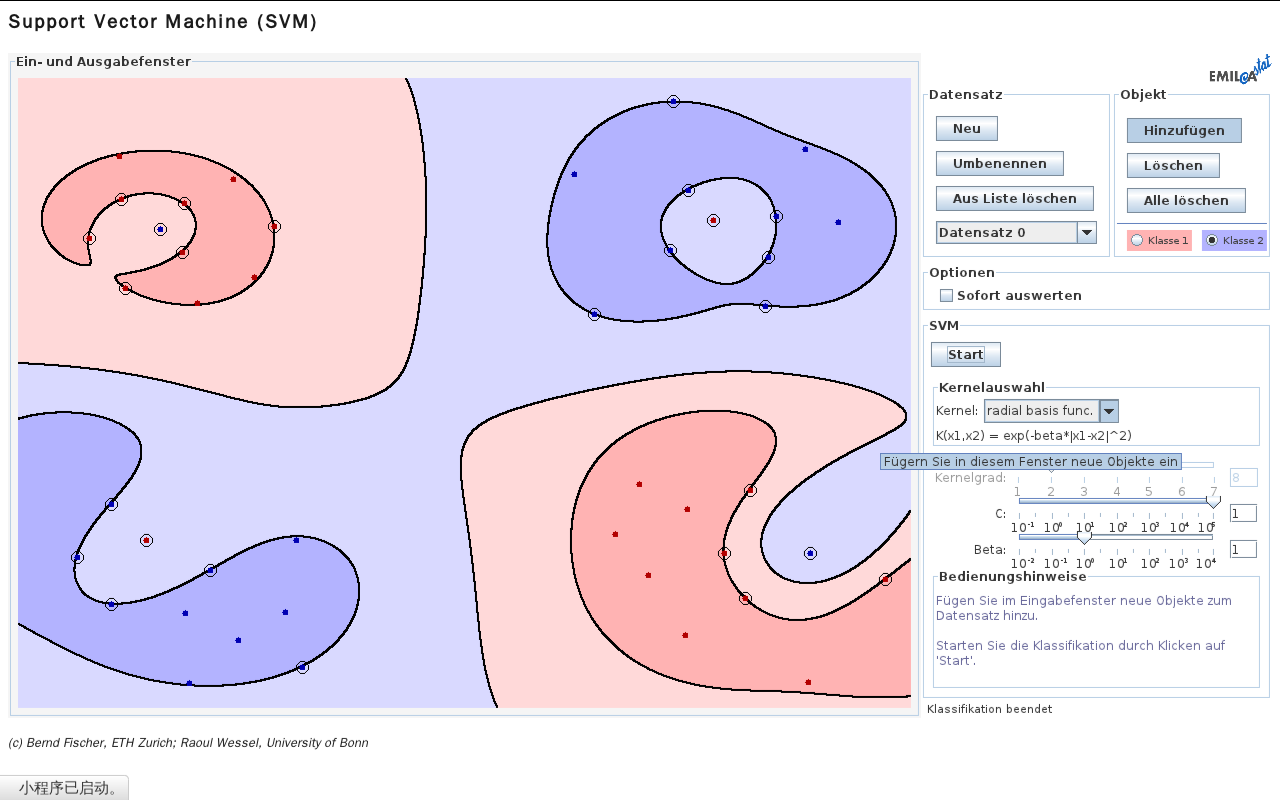
\includegraphics[width=.9\textwidth]{b-rbf-b1-c1}
\end{center}

\item 
Gaussian kernel with $\beta = 10$ and $C=1000$
\begin{center}
  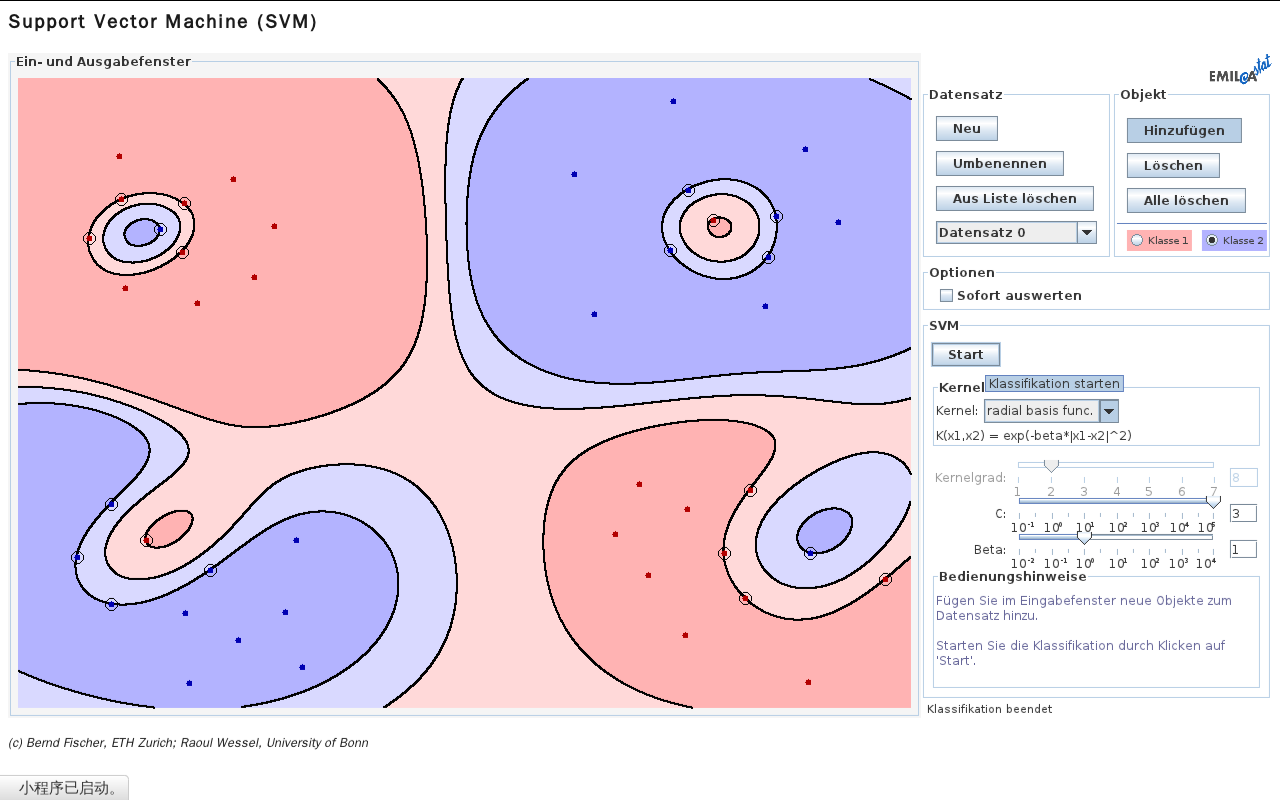
\includegraphics[width=.9\textwidth]{b-rbf-b1-c3}
\end{center}

\end{enumerate}

Paramenter $C$ controls the learning intention between overfitting and underfitting. Namely, choosing $C$ with higher value will result in better approximating the training data, while it is more sensitive to noise. On the contrary, SVM with smaller $C$ are less senstive to noise, but may not well approximate the training data.

\section{}
In Figure 2-a, the kernel function is rbf. The classification is fine. The support vectors might be as shown in the figure below.
\begin{center}
  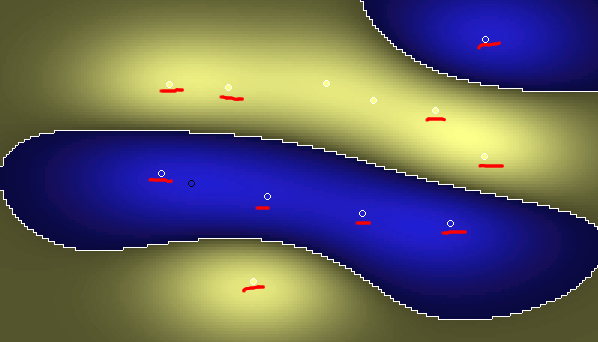
\includegraphics[width=.7\textwidth]{ex2-support-vectors}
\end{center}

In Figure 2-b, we see the classification line as a hyperbola line. Thus, the kernel function is polynomial with degree 2. We should use a higher degree kernel functions as we see the data are not well classified.

\section{}
\paragraph{Soft margin linear SVM: Primal}
\begin{align*}
  \min_{\mathbf{w}, \boldsymbol{\xi}, b} ~& \frac{1}{2} \mathbf{w}^T\mathbf{w} + \frac{C}{n} \boldsymbol{\xi}^T\mathbf{1}_n & \\
  & y_i(\mathbf{w}^T \mathbf{x}_i - b) \ge 1 - \xi_i,& i = 1, \dots, n \\
  & \xi_i \ge 0,& i = 1, \dots, n
\end{align*}

\paragraph{Soft margin linear SVM: Dual}
\begin{align*}
  \max_{\boldsymbol{\alpha}} ~& \boldsymbol{\alpha}^T \mathbf{1}_n - \frac{1}{2} \boldsymbol{\alpha}^T G \boldsymbol{\alpha} & \\
  & \boldsymbol{\alpha}^T \mathbf{y} = 0 & \\
  & 0 \le \alpha_i \le \frac{C}{n} & i = 1, \dots, n
\end{align*}
where $G \in \mathbb{R}^n \times \mathbb{R}^n, G_{ij} = y_i y_j \mathbf{x}_i^T \mathbf{x}_j$.

\paragraph{Kernel SVM: Primal}
\begin{align*}
  \min_{\mathbf{w}, \boldsymbol{\xi}, b} ~& \frac{1}{2} \mathbf{w}^T\mathbf{w} + \frac{C}{n} \boldsymbol{\xi}^T\mathbf{1}_n & \\
  & y_i(\mathbf{w}^T \boldsymbol{\Phi}(\mathbf{x}_i) - b) \ge 1 - \xi_i,& i = 1, \dots, n \\
  & \xi_i \ge 0,& i = 1, \dots, n
\end{align*}

\paragraph{Kernel SVM: Dual}
\begin{align*}
  \max_{\boldsymbol{\alpha}} ~& \boldsymbol{\alpha}^T \mathbf{1}_n - \frac{1}{2} \boldsymbol{\alpha}^T G \boldsymbol{\alpha} & \\
  & \boldsymbol{\alpha}^T \mathbf{y} = 0 & \\
  & 0 \le \alpha_i \le \frac{C}{n} & i = 1, \dots, n
\end{align*}
where $G \in \mathbb{R}^n \times \mathbb{R}^n, G_{ij} = y_i y_j k(\mathbf{x}_i, \mathbf{x}_j)$.

\section{}
\begin{itemize}
\item $K=\alpha K_1$ for $\alpha > 0$ is a valid kernel.

\[ K(x, y) = \alpha K_1(x, y) = \alpha K_1(y, x) = K(x, y) \]

For all $n \ge 1, x_1 \dots x_n \in \mathcal{X}, c_1 \dots c_n \in \mathbb{R}$:
\begin{align*}
  \sum_{i,j} c_i c_j K(x_i, x_j) & = \sum_{i,j} c_i c_j \alpha K_1(x_i, x_j) \\
   & = \alpha \sum_{i,j} c_i c_j K_1(x_i, x_j) \\
   & \ge 0
\end{align*}

\item $K= K_1 + K_2$ is a valid kernel.

\[ K(x, y) = K_1(x, y) + K_2(x, y) = K_1(y, x) + K_2(y, x) = K(x, y) \]

For all $n \ge 1, x_1 \dots x_n \in \mathcal{X}, c_1 \dots c_n \in \mathbb{R}$:
\begin{align*}
  \sum_{i,j} c_i c_j K(x_i, x_j) & = \sum_{i,j} c_i c_j (K_1(x_i, x_j) + K_2(x_i, x_j)) \\
   & = \sum_{i,j} c_i c_j K_1(x_i, x_j) + \sum_{i,j} c_i c_j K_2(x_i, x_j) \\
   & \ge 0
\end{align*}

\item $K= K_1 - K_2$ is not a valid kernel.

  Counterexample: $K_1(\mathbf{x}, \mathbf{y}) = \mathbf{x}^T\mathbf{y}$ and $K_2(\mathbf{x}, \mathbf{y}) = 2\mathbf{x}^T\mathbf{y}$. Both $K_1$ and $K_2$ are kernel functions. However, $K(\mathbf{x}, \mathbf{y}) = K_1(\mathbf{x}, \mathbf{y}) - K_2(\mathbf{x}, \mathbf{y}) = -\mathbf{x}^T\mathbf{y}$ is not a valid kernel. If we choose $n = 1, x_1 = 1, c_1 = 1$,
  \[ \sum_{i,j} c_i c_j K(x_i, x_j) = -1 < 0 \]

\item $K(x,y) =f(x)K_1(x,y)f(y)$ for any functions $f : \mathcal{X} \rightarrow \mathbb{R}$, is a valid kernel.

\[ K(x, y) = f(x)K_1(x,y)f(y) = f(y)K_1(y,x)f(x) = K(x, y) \]

For all $n \ge 1, x_1 \dots x_n \in \mathcal{X}, c_1 \dots c_n \in \mathbb{R}$:
\begin{align*}
  \sum_{i,j} c_i c_j K(x_i, x_j) & = \sum_{i,j} c_i c_j f(x_i) K_1(x_i, x_j) f(x_j) \\
   & = \sum_{i,j} (c_i f(x_i)) (c_j f(x_j)) K_1(x_i, x_j) \\
   & \ge 0
\end{align*}

\end{itemize}

\section{}
\begin{align*}
  \boldsymbol{\Phi}(\mathbf{x})^T \boldsymbol{\Phi}(\mathbf{y}) &= 1 + 2x_1y_1 + 2x_2y_2 + x_1^2y_1^2 + x_2^2y_2^2 + 2x_1x_2y_1y_2 \\
  &= (1 + x_1y_1 + x_2y_2)^2 \\
  &= (1 + \mathbf{x}^T\mathbf{y}) ^ 2 \\
  &= K(\mathbf{x}, \mathbf{y})
\end{align*}

If the input is from $\mathbb{R}^n$, expanding $\mathbf{x}^T\mathbf{y} + 1$, we have $n+1$ terms. The square of it would have \[ n + 1 + \frac{(n+1)n}{2} = \frac{(n+1)(n+2)}{2} \] terms. Therefore, the correspoinding feature space would be $\frac{(n+1)(n+2)}{2}$ dimensions.

\section{}

\end{document}
